\documentclass{article}

\usepackage{graphicx}
\usepackage{geometry}

\newcommand\tab[1][5mm]{\hspace*{#1}}

\geometry{lmargin=30mm, rmargin=30mm}
 \begin{document}
 	\title{COM S 342\large \\Homework 1}
	\author{Christian Shinkle}
	\maketitle
	\begin{enumerate}
		\item 
		\begin{enumerate}
			\item The terminals are $-, *, a$. The non-terminal is $S$.
			\item 
			\item
			\item 
			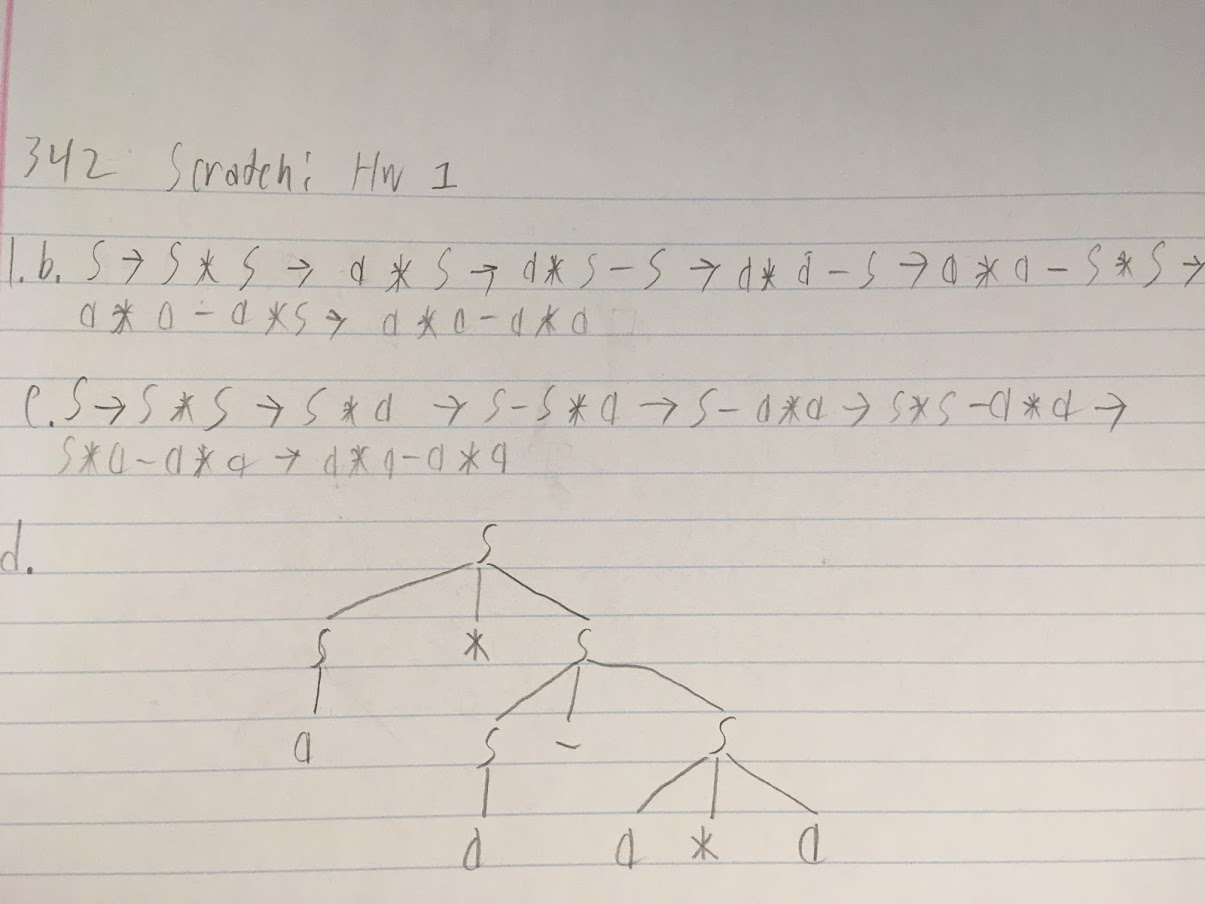
\includegraphics[width=4cm]{1bcd.jpg}
			\item No, the left derviation will produce a different parse tree then the right derviation.
			\item Three strings that don't belong to the language are:
			\begin{itemize}
				\item $a*b$
				\item $a*c$
				\item $d-a$
			\end{itemize}
		\end{enumerate}
		\item 
		\begin{enumerate}
			\item The grammar is ambiguous because there are two disticnt parse that can be created using the production rule $E\rightarrow E+T|E*T|T$. If you are given a string $x+y*z$, you can create a derivation by either deriving the $x+y$ first or the $y*z$ first.
			\item
			\item 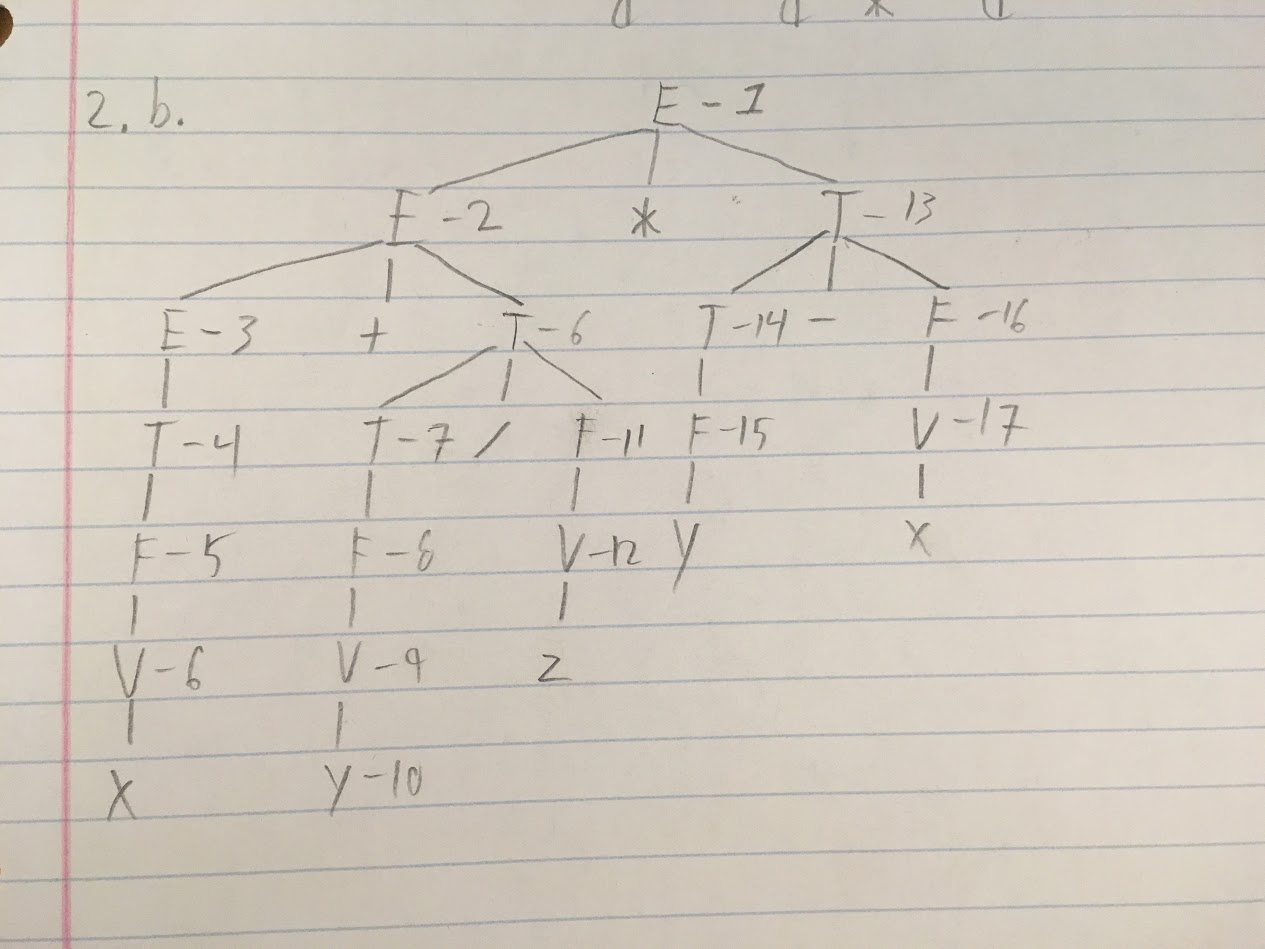
\includegraphics[width=4cm]{2b.jpg}
		\end{enumerate}
		\item 
		\begin{enumerate}
			\item The associativity of @, !, and $<$ is $<$ first, followed by !, then @ last because $<$ is derived from $G$ and $G$ is derived from $F$, which also derives !, and $F$ is derived from $E$, which also derives @. In layman's terms, you can't make an @ until you have made all the !, and you can't make a ! until you have made all the $<$.
			\item $<$ will always take precedence over ! and ! will always take precedence over @ because, again, $<$ is derived from $G$ and $G$ is derived from $F$ and $F$ is derived from $E$.
			\item 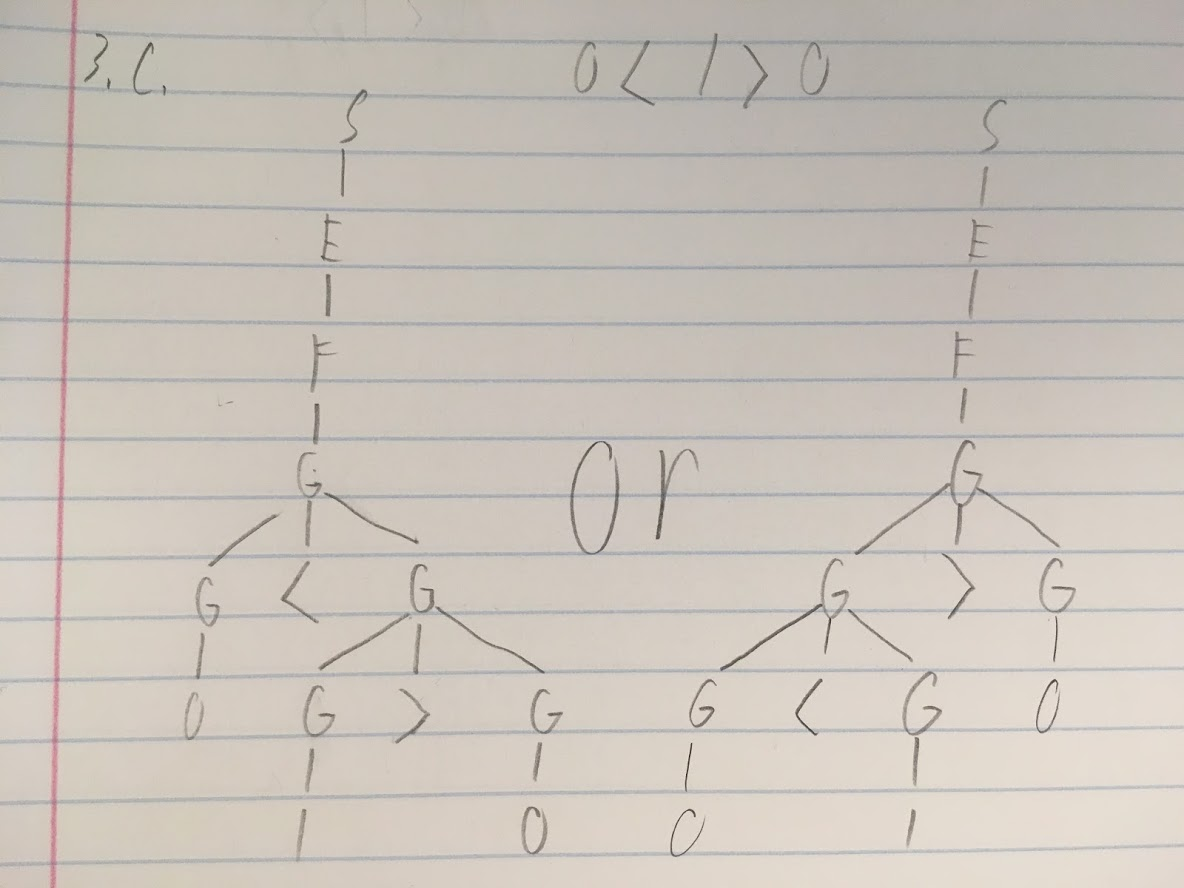
\includegraphics[width=4cm]{3c.jpg}
		\end{enumerate}
		\item The production rules of the grammar where $S$ is the start variable: \\
		$V\ \rightarrow\ V@X|V.X|X$\\
		$X\ \rightarrow\ X\times Y|Y$\\
		$Y\ \rightarrow\ Z\cup Y|Z\cap Y|Z$\\
		$Z\ \rightarrow\ \neg Z|a|b|c|true|false$
		\item For Python:
		\begin{itemize}
			\item The ``compound\_stmt'' and the ``async\_stmt'' can accept the ``for\_stmt.''
			\item Consider the following script:\\ 
			1. i = 5;\\
			2. while i != 0:\\
			3. \tab print(i);\\
			4. \tab i -= 1;\\
			5. print("Blast off!");\\
			Line 1 is a simple\_stmt derived from a small\_stmt derived from a expr\_stmt. This is how assignment statements are handled.\\
			Line 2 is a compound\_stmt derived from a while\_stmt which uses a ``test'' followed by a `:' followed by a suite.\\
			Line 3 is the first suite which is a NEWLINE character, an INDENT character, and a stmt. The stmt is derived from a compound\_stmt derived from a funcdef that print `i'.\\
			Line 4 is the second suite which is a simple\_stmt derived from a small\_stmt derived from expr\_stmt derived from an augassign which uses `-=' to decrement `i' by one.\\
			Line 5 is the same derivation as line 3 except there is no suite with a NEWLINE character and INDENT character, the derivations starts at a compount\_stmt.
		\end{itemize}
	\end{enumerate}
 \end{document}